\thispagestyle{hoccungpinone}
\pagestyle{hoccungpi}
\everymath{\color{hoccungpi}}
\graphicspath{{../hoccungpi/pic/}}
\blfootnote{\color{hoccungpi}\color{hoccungpi}$^1$Giáo viên Toán trường THPT chuyên Lê Hồng Phong, Nam Định.}
\begingroup
\AddToShipoutPicture*{\put(0,616){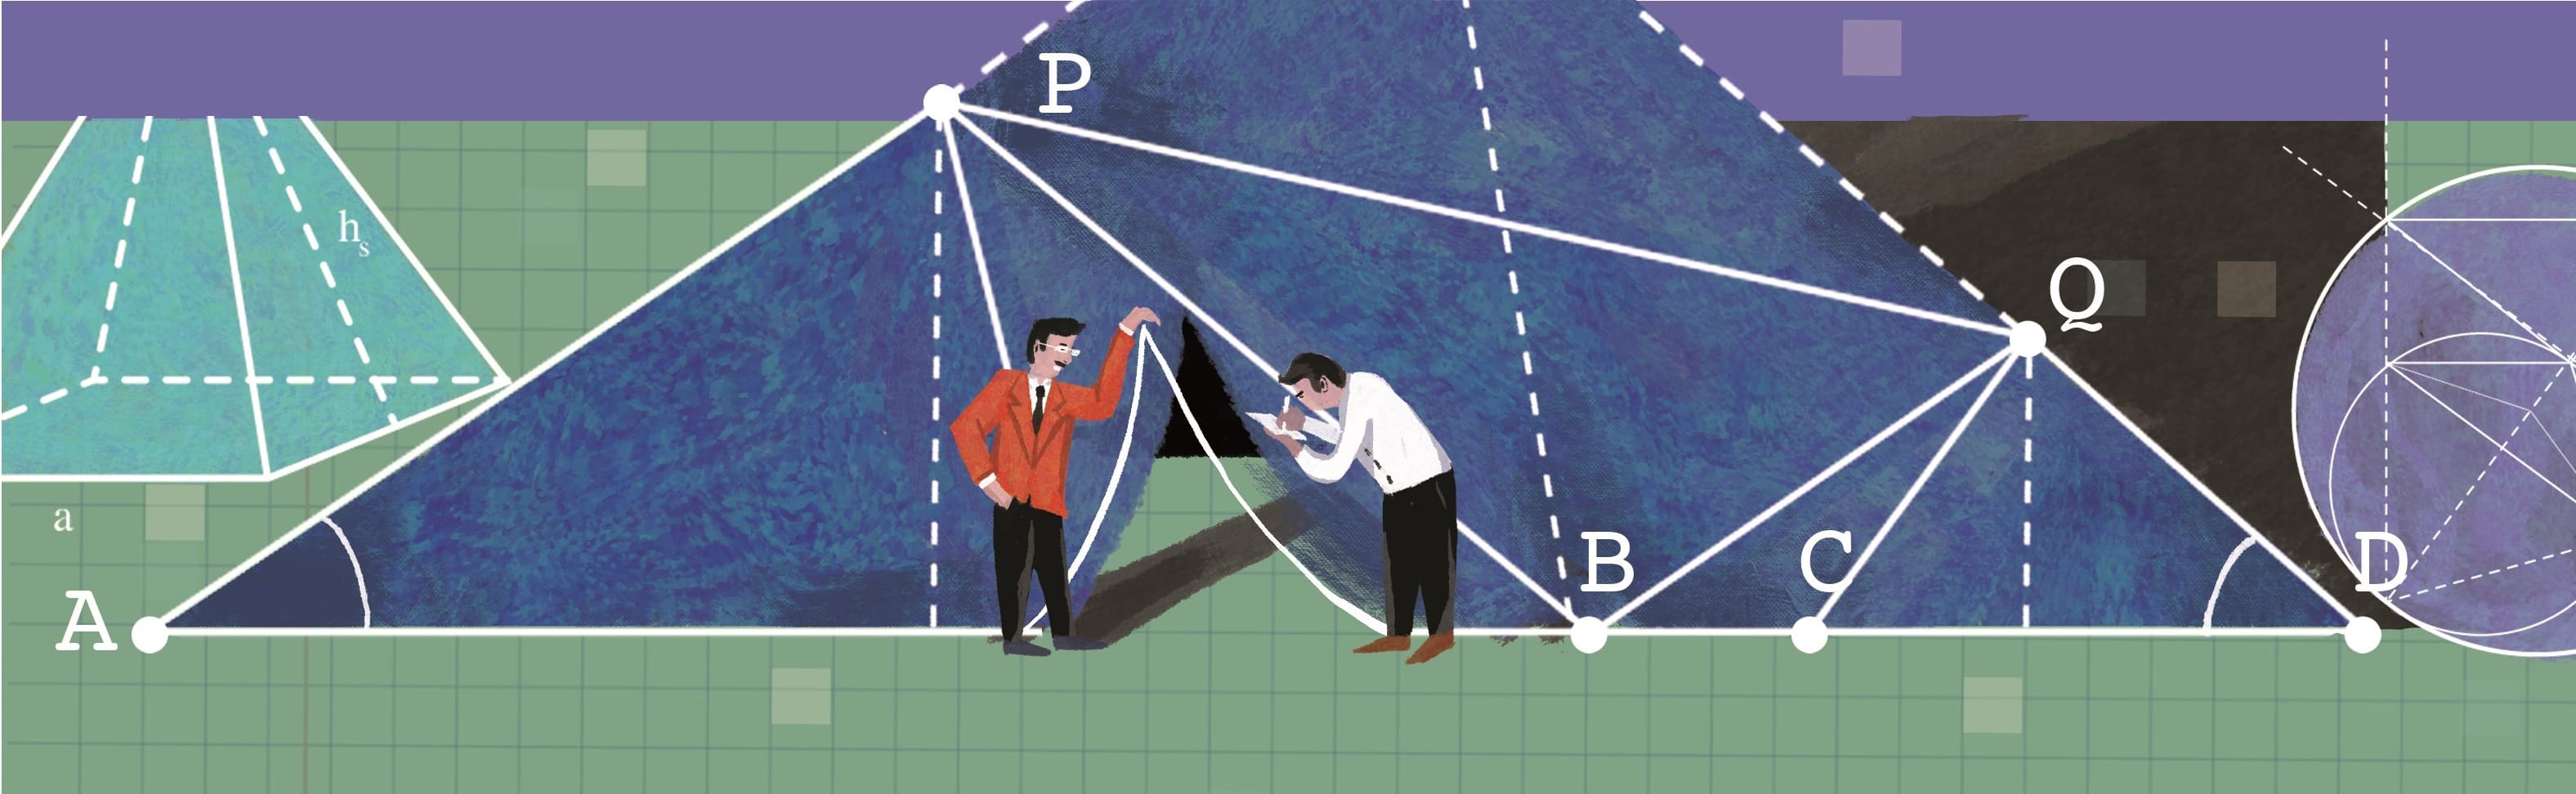
\includegraphics[width=19.3cm]{../bannerhoccungpi}}}
\AddToShipoutPicture*{\put(58,520){
\includegraphics[scale=1]{../tieude.pdf}}}
\centering
\endgroup
\vspace*{190pt}

\textit{Có thể nói rằng, sự ra đời của lý thuyết đồ thị được đánh dấu bằng bài báo \textit{bảy cây cầu ở thành phố Königsberg} của Leonhard Euler. Trải qua hàng trăm năm, lý thuyết đồ thị đã trở thành một mảng kiến thức đồ sộ, là một trong những công cụ mạnh, được sử dụng nhiều trong cả hai phân môn Toán lý thuyết và Toán ứng dụng. Trong bài viết này, chúng tôi trình bày ngắn gọn một số kiến thức cơ sở của lý thuyết đồ thị, và một số ví dụ trong việc xây dựng mô hình đồ thị. Sau đó, chúng tôi giới thiệu hai cấu trúc đồ thị đặc biệt và một số bài tập liên quan.}
\begin{multicols}{2}
	\textbf{\color{hoccungpi}Sơ lược về lý thuyết đồ thị}
	\begin{figure}[H]
		\vspace*{-5pt}
		\centering
		\captionsetup{labelformat= empty, justification=centering}
		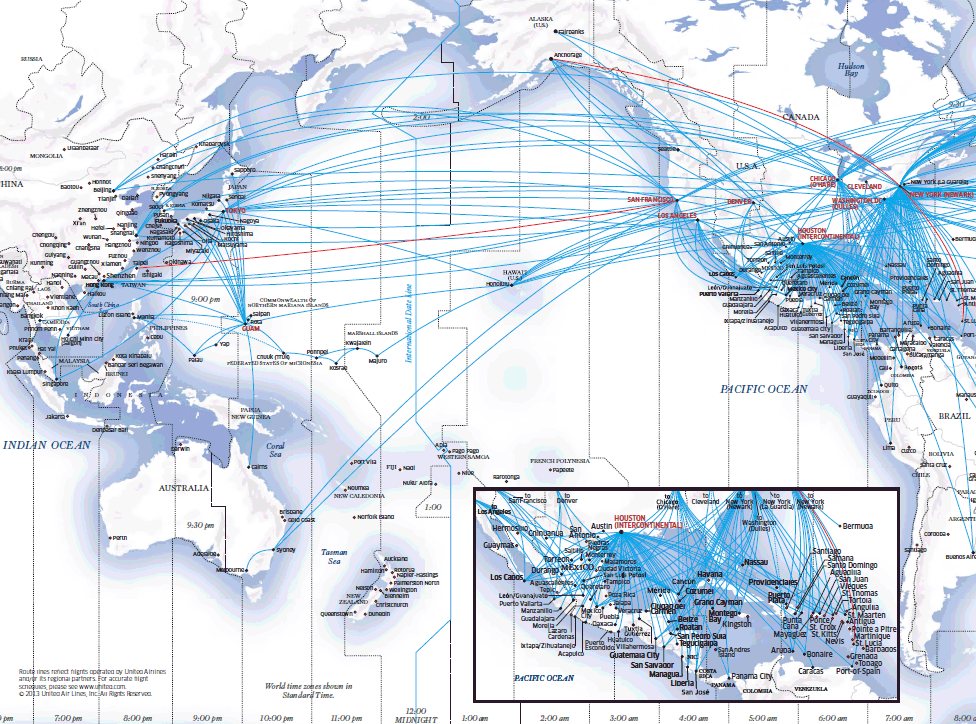
\includegraphics[width= 1\linewidth]{United_Airlines_asia_pacific}
		\caption{\small\textit{\color{hoccungpi}Hình $1$. Bản đồ các đường bay ở Châu Á -- Thái Bình Dương của hãng hàng không United Airlines.}}
		\vspace*{-10pt}
	\end{figure}
	Lý thuyết đồ thị có lịch sử phát triển lâu dài từ thế kỷ $18$. Càng ngày, người ta càng thấy nhiều ứng dụng của lý thuyết đồ thị trong nhiều lĩnh vực của cuộc sống như giao thông, y sinh, tin học, thiên văn\dots. Hình $1$\footnote[2]{\url{https://www.airlineroutemaps.com/maps}} là bản đồ các tuyến đường bay của hãng hàng không United Airlines ở khu vực Châu Á -- Thái Bình Dương.
	\vskip 0.1cm
	Trong hình này, nếu ta coi mỗi sân bay như một điểm, và mỗi đường bay như một cạnh nối hai điểm, thì đây chính là một mô hình bao gồm hai tập hợp: tập hợp điểm, và tập hợp cạnh thể hiện mối liên hệ giữa các điểm. Trong cả lý thuyết và thực tế, đôi khi ta gặp những mô hình có thể biểu diễn thông qua mô hình hai tập hợp này. Những mô hình như vậy đều có thể coi là một mô hình đồ thị. Ta đi đến định nghĩa sau về đồ thị (vô hướng): 
	\vskip 0.1cm
	\textbf{\color{hoccungpi}Định nghĩa} $\pmb{1.1}$ (Đồ thị)\textbf{\color{hoccungpi}.}
		Một \textit{đồ thị} là một tập hợp các điểm (gọi là các \textit{đỉnh} của đồ thị), và một tập hợp các đoạn (gọi là \textit{cạnh} của đồ thị), sao cho mỗi đoạn này đều có hai đầu mút là hai đỉnh của đồ thị. 
	\vskip 0.1cm
	Theo định nghĩa $1.1$, ta thấy rằng mỗi đồ thị $\pazocal{G}$ là một bộ $(V,E)$ gồm hai tập hợp: tập đỉnh $V$ và tập cạnh $E$. Vì vậy, ta thường ký hiệu đồ thị $\pazocal{G} = (V,E)$. Ta có một số lưu ý sau:  
	\vskip 0.1cm
	$\bullet$ Mỗi đồ thị không có khuyên (cạnh tự nối), và hai đỉnh bất kỳ được nối với nhau bằng nhiều nhất một cạnh gọi là một đồ thị đơn giản, hay ngắn gọn là \textit{đồ thị đơn}. Ngược lại, đồ thị mà giữa hai đỉnh có thể có nhiều hơn một cạnh được gọi là đa đồ thị.
	\vskip 0.1cm
	$\bullet$ Trong bài viết này, khi nói đến ``đồ thị'', nếu không có lưu ý gì, ta hiểu đó là một đồ thị đơn và hữu hạn (nghĩa là tập đỉnh và tập cạnh là các tập hữu hạn).
	\vskip 0.1cm
	Ta kết thúc phần này với một số định nghĩa, và một kết quả quen thuộc\footnote[3]{\color{hoccungpi}Một số khái niệm như đường đi có thể được định nghĩa hơi khác nhau giữa các tài liệu khác nhau (chú thích của BBT).}. 
	\vskip 0.1cm
	\textbf{\color{hoccungpi}Định nghĩa} $\pmb{1.2}$ (Một số định nghĩa quan trọng)\textbf{\color{hoccungpi}.}
	\vskip 0.1cm
	$1.$ Một đỉnh của đồ thị có \textit{bậc} $n$ nếu nó là đầu mút của $n$ cạnh trong đồ thị. Ký hiệu bậc của  đỉnh $v$ là deg$(v)$. 
	\vskip 0.1cm
	$2.$ Một \textit{đường đi} trên đồ thị là một dãy các đỉnh $u_1, u_2, \dots,u_k$ sao cho giữa hai đỉnh liên tiếp $u_i,u_{i+1}$ trong dãy đều có một cạnh của đồ thị nối chúng. Đường đi trong đó mỗi đỉnh chỉ được đi qua nhiều nhất một lần gọi là \textit{đường đi đơn}.
	\vskip 0.1cm
	$3.$ Đồ thị $\pazocal{G}$ được gọi là \textit{liên thông} nếu với hai đỉnh $u,v$ tùy ý, tồn tại một đường đi từ $u$ đến $v$.
	\vskip 0.1cm
	$4.$ Một \textit{chu trình} là một đường đi mà đỉnh xuất phát trùng với đỉnh kết thúc. Chu trình đi qua tất cả các đỉnh của đồ thị, mỗi đỉnh đúng một lần  được gọi là \textit{chu trình Hamilton}. Chu trình đi qua tất cả các cạnh của đồ thị, mỗi cạnh đúng một lần được gọi là \textit{chu trình Euler}.
	\vskip 0.1cm
	$5.$ \textit{Đồ thị đầy đủ} là đồ thị mà giữa hai đỉnh bất kỳ đều có một cạnh nối. 
	\vskip 0.1cm
	$6.$ Đồ thị $G$ gọi là một \textit{đồ thị con} của đồ thị $\pazocal{G}$ nếu tập đỉnh và tập cạnh của đồ thị $G$ lần lượt là tập con của tập đỉnh và tập cạnh của đồ thị $\pazocal{G}$.
	\vskip 0.1cm
	$7.$ Một \textit{thành phần liên thông} của một đồ thị là một đồ thị con trong đó giữa bất kỳ hai đỉnh nào đều có đường đi đến nhau, và không thể nhận thêm bất kỳ một đỉnh hoặc một cạnh nào mà vẫn duy trì tính chất trên. Ta thấy ngay rằng một đồ thị bất kỳ có thể được phân tích một cách duy nhất thành hợp rời của các  thành phần liên thông. 
	\vskip 0.1cm
	\textbf{\color{hoccungpi}Bổ đề} $\pmb{1.1}$ (Bổ đề bắt tay)\textbf{\color{hoccungpi}.}
		Cho đồ thị $\pazocal{G} = (V,E)$. Khi đó:
		\begin{align*}
			\sum\limits_{v \in V} deg(v) = 2 |E|.
		\end{align*}
	Việc chứng minh bổ đề không có gì là khó khăn và ta thu được ngay một hệ quả là: số đỉnh bậc lẻ trong mọi đồ thị luôn là một số chẵn. 
	\vskip 0.1cm
	$\pmb{2.}$ \textbf{\color{hoccungpi}Phát hiện và sử dụng mô hình đồ thị}
	\vskip 0.1cm
	Kỹ năng đầu tiên cần rèn luyện khi sử dụng lý thuyết đồ thị là phát hiện được mô hình. Trong rất nhiều bài toán, ý tưởng về một mô hình đồ thị được ẩn đi một cách khéo léo. Chúng ta cùng xét một số ví dụ.
	\vskip 0.1cm
	\textbf{\color{hoccungpi}Ví dụ} $\pmb{2.1}$ (Olympic Ấn Độ năm $2023$)\textbf{\color{hoccungpi}.} Cho $\pazocal{S}$ là một tập hợp gồm hữu hạn số nguyên dương. Giả sử rằng có đúng $2023$ cặp $(x,y)$ trong $\pazocal{S} \times \pazocal{S}$, sao cho tích $xy$ là số chính phương. Chứng minh rằng có thể tìm được ít nhất bốn số phân biệt trong $\pazocal{S}$ sao cho tích của hai số bất kỳ trong bốn số này không là số chính phương.
	\vskip 0.1cm
	\textit{Lời giải.} Ta xây dựng đồ thị $\pazocal{G}$ với tập đỉnh chính là tập $\pazocal{S}$, hai đỉnh $x,y$ của nó được nối với nhau bằng một cạnh nếu $xy$ là số chính phương. Ta có nhận xét quan trọng sau: nếu $x-y$ và $y-z$ là hai cạnh của đồ thị thì $x-z$ cũng là cạnh của đồ thị. Thật vậy, nếu $xy = a^2, yz = b^2$ thì $xz = (ab)^2 / y^2$. Bạn đọc có thể chứng minh được rằng vế phải là một số chính phương, do đó $xz$ cũng là số chính phương. 
	\vskip 0.1cm
	Từ nhận xét trên, ta thấy ngay cấu trúc của đồ thị $\pazocal{G}$ là như sau: nó gồm các thành phần liên thông mà mỗi thành phần liên thông là một đồ thị đầy đủ. Từ đây, bài toán quy về chứng minh đồ thị $\pazocal{G}$ có ít nhất bốn thành phần liên thông. Thật vậy, giả sử $\pazocal{G}$ có ít hơn bốn thành phần liên thông, ta gọi số đỉnh của các thành phần liên thông này là $a_1, a_2, a_3$ (các $a_i$ có thể bằng $0$). Mỗi đồ thị (đơn) đầy đủ trên $a$ đỉnh có $\frac{a(a-1)}{2}$ cạnh, và mỗi cạnh đóng góp $2$ đơn vị vào  số cặp $(x, y)$ để $xy$ là một số chính phương. Tuy nhiên, ta chú ý rằng mỗi đỉnh tương ứng với số $s\in S$, mặc dù không nối với chính nó do tính đơn của đồ thị, nhưng thỏa mãn $ss$ là một số chính phương, nên cũng đóng góp $1$ đơn vị vào số cặp $(x, y)$ để $xy$ là một số chính phương. Chính vì vậy, mỗi thành phần liên thông trên $a$ đỉnh có $a(a-1)+a=a^2$ cặp $(x,y)$ như vậy. Suy ra số cặp $(x,y)$ trong $\pazocal{S} \times \pazocal{S}$, sao cho tích $xy$ là một số chính phương bằng
	\begin{align*}
		a_1^2 + a_2^2 + a_3^2 =2023.
	\end{align*}
	Mặt khác, một số chính phương khi chia cho $8$ có số dư thuộc tập hợp $\{0;1;4\}$. Do đó, vế trái là tổng của ba số chính phương, nên không thể chia $8$ dư $7$, trong khi đó $2023$ chia $8$ dư $7$. Điều này là mâu thuẫn!   
	\vskip 0.1cm
	\textbf{\color{hoccungpi}Ví dụ} $\pmb{2.2}$ (Bài toán dự tuyển thi IMO năm $2018$, Armenia đề xuất)\textbf{\color{hoccungpi}.}
	Queenie và Horst chơi một trò chơi trên một bàn cờ kích thước $20 \times 20$. Ban đầu, bàn cờ chưa có quân cờ nào. Ở mỗi lượt đi, Horst đặt một quân mã đen vào một ô còn trống sao cho quân mã này không thể ăn được bất cứ quân mã nào đã đặt trước đó; sau đó, Queenie đặt một quân hậu vào một ô trống tùy ý. Trò chơi kết thúc khi một trong hai người không thể đặt thêm quân lên bàn cờ. Tìm số nguyên dương $K$ lớn nhất sao cho với mọi chiến thuật chơi của Queenie, Horst có thể đặt được ít nhất $K$ quân mã lên bàn cờ.  
	\vskip 0.1cm
	\textit{Lời giải.}
	Ta chỉ ra giá trị lớn nhất của $K$ là $K=100$ qua hai bước. Đầu tiên, ta chỉ ra một chiến lược mà Host có thể đặt được ít nhất $100$ quân mã lên bàn cờ. Sau đó, ta chỉ ra một chiến lược của Queenie mà Horst không thể đặt quá $100$ quân mã lên bàn cờ.
	\vskip 0.1cm
	\textbf{\color{hoccungpi}Chiến lược của Horst.} Ta tô màu đen, trắng các ô của bàn cờ một cách đan xen như bàn cờ vua thông thường. Horst chỉ cần lần lượt đặt các quân mã lên một ô đen còn trống. Để ý rằng bàn cờ có $20\cdot 20/2 = 200$ ô đen và hai con mã ở hai ô cùng màu không thể ăn nhau. Do sau mỗi lượt đi, số ô đen còn trống giảm đi không quá $2$ nên trò chơi chỉ kết thúc sau ít nhất $100$ lượt đi và vì thế Horst có thể đặt được $100$ quân mã.
	\vskip 0.1cm
	\textbf{\color{hoccungpi}Chiến lược của Queenie.} Xét một bảng con $4 \times 4$ của bảng $20 \times 20$ ban đầu. Coi mỗi ô vuông đơn vị như một đỉnh đồ thị, hai đỉnh được nối với nhau khi và chỉ khi con mã có thể đi từ ô nọ đến ô kia sau một nước đi. Khi đó, trong bảng $4 \times 4$, ta xây dựng được $4$ chu trình có độ dài $4$ như hình minh họa. Chú ý rằng mỗi ô trong bảng $4\times 4$ nằm trên đúng một chu trình. Chia bảng $20 \times 20$ thành $25$ bảng $4 \times 4$ và xây dựng các chu trình như trên. Như vậy, ta thu được $100$ chu trình có độ dài $4$. 
	\begin{figure}[H]
		\vspace*{-5pt}
		\centering
		\definecolor{qqqqff}{rgb}{0.,0.,1.}
		\begin{tikzpicture}[scale=0.9, hoccungpi]
			\fill[fill=black,fill opacity=0.5] (6.,11.) -- (7.,11.) -- (7.,10.) -- (6.,10.) -- cycle;
			\fill[fill=black,fill opacity=0.5] (8.,11.) -- (8.,10.) -- (9.,10.) -- (9.,11.) -- cycle;
			\fill[fill=black,fill opacity=0.5] (7.,10.) -- (8.,10.) -- (8.,9.) -- (7.,9.) -- cycle;
			\fill[fill=black,fill opacity=0.5] (9.,10.) -- (10.,10.) -- (10.,9.) -- (9.,9.) -- cycle;
			\fill[fill=black,fill opacity=0.5] (8.,9.) -- (9.,9.) -- (9.,8.) -- (8.,8.) -- cycle;
			\fill[fill=black,fill opacity=0.5] (6.,9.) -- (7.,9.) -- (7.,8.) -- (6.,8.) -- cycle;
			\fill[fill=black,fill opacity=0.5] (7.,8.) -- (8.,8.) -- (8.,7.) -- (7.,7.) -- cycle;
			\fill[fill=black,fill opacity=0.5] (9.,8.) -- (10.,8.) -- (10.,7.) -- (9.,7.) -- cycle;
			\draw [line width=1.2pt] (6.,11.)-- (10.,11.);
			\draw (6.,10.)-- (10.,10.);
			\draw (6.,9.)-- (10.,9.);
			\draw (6.,8.)-- (10.,8.);
			\draw [line width=1.2pt] (6.,7.)-- (10.,7.);
			\draw [line width=1.2pt] (6.,11.)-- (6.,7.);
			\draw (7.,11.)-- (7.,7.);
			\draw (8.,11.)-- (8.,7.);
			\draw (9.,11.)-- (9.,7.);
			\draw [line width=1.2pt] (10.,11.)-- (10.,7.);
			\draw (6.,11.)-- (7.,11.);
			\draw (7.,11.)-- (7.,10.);
			\draw (7.,10.)-- (6.,10.);
			\draw (6.,10.)-- (6.,11.);
			\draw (8.,11.)-- (8.,10.);
			\draw (8.,10.)-- (9.,10.);
			\draw (9.,10.)-- (9.,11.);
			\draw (9.,11.)-- (8.,11.);
			\draw (7.,10.)-- (8.,10.);
			\draw (8.,10.)-- (8.,9.);
			\draw (8.,9.)-- (7.,9.);
			\draw (7.,9.)-- (7.,10.);
			\draw (9.,10.)-- (10.,10.);
			\draw (10.,10.)-- (10.,9.);
			\draw (10.,9.)-- (9.,9.);
			\draw (9.,9.)-- (9.,10.);
			\draw (8.,9.)-- (9.,9.);
			\draw (9.,9.)-- (9.,8.);
			\draw (9.,8.)-- (8.,8.);
			\draw (8.,8.)-- (8.,9.);
			\draw (6.,9.)-- (7.,9.);
			\draw (7.,9.)-- (7.,8.);
			\draw (7.,8.)-- (6.,8.);
			\draw (6.,8.)-- (6.,9.);
			\draw (7.,8.)-- (8.,8.);
			\draw (8.,8.)-- (8.,7.);
			\draw (8.,7.)-- (7.,7.);
			\draw (7.,7.)-- (7.,8.);
			\draw (9.,8.)-- (10.,8.);
			\draw (10.,8.)-- (10.,7.);
			\draw (10.,7.)-- (9.,7.);
			\draw (9.,7.)-- (9.,8.);
			\draw (6.483008725199413,10.519186248976789)-- (7.483057165045717,8.490516556717143);
			\draw (6.483008725199413,10.519186248976789)-- (8.51167841745906,9.533424215414003);
			\draw (8.51167841745906,9.533424215414003)-- (9.468867638454808,7.519040929437875);
			\draw (9.468867638454808,7.519040929437875)-- (7.483057165045717,8.490516556717143);
			\draw (7.497343571329236,10.50489984269327)-- (6.468722318915894,8.533375775567698);
			\draw (6.468722318915894,8.533375775567698)-- (8.49739201117554,7.504754523154356);
			\draw (8.49739201117554,7.504754523154356)-- (9.497440451021845,9.490564996563448);
			\draw (9.497440451021845,9.490564996563448)-- (7.497343571329236,10.50489984269327);
			\draw (8.49739201117554,10.547759061543827)-- (6.468722318915894,9.533424215414003);
			\draw (6.468722318915894,9.533424215414003)-- (7.483057165045717,7.504754523154356);
			\draw (7.483057165045717,7.504754523154356)-- (9.511726857305364,8.51908936928418);
			\draw (9.511726857305364,8.51908936928418)-- (8.49739201117554,10.547759061543827);
			\draw (9.483154044738328,10.50489984269327)-- (7.468770758762199,9.533424215414003);
			\draw (7.468770758762199,9.533424215414003)-- (6.4972951314829315,7.490468116870837);
			\draw (6.4972951314829315,7.490468116870837)-- (8.483105604892023,8.533375775567698);
			\draw (8.483105604892023,8.533375775567698)-- (9.483154044738328,10.50489984269327);
			\begin{scriptsize}
				\draw [fill=qqqqff] (6.5,10.5) circle (2.5pt);
				\draw [fill=qqqqff] (7.56,10.5) circle (2.5pt);
				\draw [fill=qqqqff] (8.5,10.5) circle (2.5pt);
				\draw [fill=qqqqff] (9.5,10.5) circle (2.5pt);
				\draw [fill=qqqqff] (9.5,9.5) circle (2.5pt);
				\draw [fill=qqqqff] (9.5,8.5) circle (2.5pt);
				\draw [fill=qqqqff] (9.5,7.5) circle (2.5pt);
				\draw [fill=qqqqff] (8.5,9.5) circle (2.5pt);
				\draw [fill=qqqqff] (8.5,8.5) circle (2.5pt);
				\draw [fill=qqqqff] (8.5,7.5) circle (2.5pt);
				\draw [fill=qqqqff] (7.5,9.5) circle (2.5pt);
				\draw [fill=qqqqff] (7.5,8.5) circle (2.5pt);
				\draw [fill=qqqqff] (7.5,7.5) circle (2.5pt);
				\draw [fill=qqqqff] (6.5,9.5) circle (2.5pt);
				\draw [fill=qqqqff] (6.5,8.5) circle (2.5pt);
				\draw [fill=qqqqff] (6.5,7.5) circle (2.5pt);
			\end{scriptsize}
		\end{tikzpicture}
	\vspace*{-5pt}
	\end{figure}
	Với mỗi chu trình $A-B-C-D-A$, Quennie có thể chơi như sau. Mỗi khi Horst đặt một quân mã vào ô $A$ trong một chu trình, Queenie lập tức đặt một quân hậu vào ô $C$ đối diện ô $A$ trong chu trình. 
	\vskip 0.1cm
	Rõ ràng, sau đó Horst không thể đặt một quân mã vào ba ô $B,C,D$. Do đó, nếu Queenie chơi theo chiến lược này thì Horst chỉ đặt được tối đa $100$ quân mã lên bàn cờ.
	\vskip 0.1cm
	Tóm lại, số quân mã nhiều nhất mà Horst có thể đặt được lên bàn cờ là $K=100$.
	\begin{figure}[H]
		\vspace*{5pt}
		\centering
		\definecolor{zzttqq}{rgb}{0.6,0.2,0.}
		\definecolor{cqcqcq}{rgb}{0.7529411764705882,0.7529411764705882,0.7529411764705882}
		\begin{tikzpicture}[scale=0.35,hoccungpi, node font=\small]
			\fill[color=zzttqq,fill=zzttqq,fill opacity=0.10000000149011612] (18.,22.) -- (20.,22.) -- (20.,24.) -- (18.,24.) -- cycle;
			\fill[color=zzttqq,fill=zzttqq,fill opacity=      0.10000000149011612] (10.,18.) -- (12.,18.) -- (12.,20.) -- (10.,20.) -- cycle;
			\fill[color=zzttqq,fill=zzttqq,fill opacity=0.10000000149011612] (26.,18.) -- (28.,18.) -- (28.,20.) -- (26.,20.) -- cycle;
			\fill[color=zzttqq,fill=zzttqq,fill opacity=0.10000000149011612] (18.,14.) -- (20.,14.) -- (20.,16.) -- (18.,16.) -- cycle;
			\draw [color=zzttqq] (18.,22.)-- (20.,22.);
			\draw [color=zzttqq] (20.,22.)-- (20.,24.);
			\draw [color=zzttqq] (20.,24.)-- (18.,24.);
			\draw [color=zzttqq] (18.,24.)-- (18.,22.);
			\draw [color=zzttqq] (10.,18.)-- (12.,18.);
			\draw [color=zzttqq] (12.,18.)-- (12.,20.);
			\draw [color=zzttqq] (12.,20.)-- (10.,20.);
			\draw [color=zzttqq] (10.,20.)-- (10.,18.);
			\draw [color=zzttqq] (26.,18.)-- (28.,18.);
			\draw [color=zzttqq] (28.,18.)-- (28.,20.);
			\draw [color=zzttqq] (28.,20.)-- (26.,20.);
			\draw [color=zzttqq] (26.,20.)-- (26.,18.);
			\draw [color=zzttqq] (18.,14.)-- (20.,14.);
			\draw [color=zzttqq] (20.,14.)-- (20.,16.);
			\draw [color=zzttqq] (20.,16.)-- (18.,16.);
			\draw [color=zzttqq] (18.,16.)-- (18.,14.);
			\draw (18.,22.)-- (12.,20.);
			\draw (20.,22.)-- (26.,20.);
			\draw (26.,18.)-- (20.,16.);
			\draw (12.,18.)-- (18.,16.);
			\draw (8.6,19.7) node[anchor=north west] {$A$};
			\draw (28.2,19.7) node[anchor=north west] {$C$};
			\draw (18.5,25.6) node[anchor=north west] {$B$};
			\draw (18.5,14) node[anchor=north west] {$D$};
			\draw (10,19.6) node[anchor=north west] {Mã};
			\draw (25.7,19.6) node[anchor=north west] {Hậu};
		\end{tikzpicture}
		\vspace*{-15pt}
	\end{figure}
	\textbf{\color{hoccungpi}Ví dụ} $\pmb{2.3}$ (Bài toán dự tuyển thi IMO năm $2020$, Hungary đề xuất)\textbf{\color{hoccungpi}.} 
	Có $4n$ viên sỏi có khối lượng lần lượt là $1,2,\dots,4n$. Mỗi viên sỏi có một trong $n$ màu và mỗi màu có đúng $4$ viên. Chứng minh rằng có thể phân hoạch các viên sỏi thành hai tập có tổng khối lượng bằng nhau, sao cho trong mỗi tập, mỗi màu đều có đúng hai viên sỏi.  
	\vskip 0.1cm
	\textit{Lời giải.} \textit{(Dựa theo lời giải của Evan Chen.)} 
	Để ý rằng 
	\begin{align*}
		1+4n = 2+ (4n-1) = 3 + (4n-2) = \dots
	\end{align*}
	Ta đặt các viên sỏi vào $n$ hộp, mỗi hộp chứa $4$ viên sỏi cùng màu. Với mỗi số nguyên $k=1,2,\dots,2n$, ta nối một cạnh giữa viên sỏi có khối lượng $k$ với viên sỏi có khối lượng $4n+1-k$. 
	\begin{figure}[H]
		\captionsetup{labelformat= empty, justification=centering}
		\centering
		\definecolor{ffqqqq}{rgb}{1.,0.,0.}
		\definecolor{qqqqff}{rgb}{0.,0.,1.}
		\definecolor{cqcqcq}{rgb}{0.7529411764705882,0.7529411764705882,0.7529411764705882}
		\begin{tikzpicture}[scale=0.232, hoccungpi, node font=\small]
			\draw (16.,22.)-- (18.,24.);
			\draw (18.,24.)-- (18.,20.);
			\draw (18.,20.)-- (22.,20.);
			\draw (22.,20.)-- (22.,24.);
			\draw (22.,24.)-- (24.,22.);
			\draw (4.,16.)-- (6.,18.);
			\draw (6.,18.)-- (6.,14.);
			\draw (6.,14.)-- (10.,14.);
			\draw (10.,14.)-- (10.,18.);
			\draw (10.,18.)-- (12.,16.);
			\draw (8.,6.)-- (10.,8.);
			\draw (10.,8.)-- (10.,4.);
			\draw (10.,4.)-- (14.,4.);
			\draw (14.,4.)-- (14.,8.);
			\draw (14.,8.)-- (16.,6.);
			\draw (24.,6.)-- (26.,8.);
			\draw (26.,8.)-- (26.,4.);
			\draw (26.,4.)-- (30.,4.);
			\draw (30.,4.)-- (30.,8.);
			\draw (30.,8.)-- (32.,6.);
			\draw (28.,16.)-- (30.,18.);
			\draw (30.,18.)-- (30.,14.);
			\draw (30.,14.)-- (34.,14.);
			\draw (34.,14.)-- (34.,18.);
			\draw (34.,18.)-- (36.,16.);
			\draw [line width=1.pt,color=qqqqff] (19.,23.)-- (21.,23.);
			\draw [line width=1.pt,color=qqqqff] (9.,17.)-- (31.,17.);
			\draw [line width=1.pt,color=qqqqff] (7.,15.)-- (13.,7.);
			\draw [line width=1.pt,color=qqqqff] (11.,5.)-- (27.,7.);
			\draw [line width=1.pt,color=qqqqff] (29.,7.)-- (33.,15.);
			\draw [line width=1.pt,color=ffqqqq] (7.,17.)-- (19.,21.);
			\draw [line width=1.pt,color=ffqqqq] (9.,15.)-- (31.,15.);
			\draw [line width=1.pt,color=ffqqqq] (11.,7.)-- (33.,17.);
			\draw [line width=1.pt,color=ffqqqq] (21.,21.)-- (29.,5.);
			\draw [line width=1.pt,color=ffqqqq] (13.,5.)-- (27.,5.);
			\draw (17.8,19.5) node[anchor=north west] {$\text{Hộp $1$}$};
			\draw (29.5,13) node[anchor=north west] {$\text{Hộp $5$}$};
			\draw (10,3) node[anchor=north west] {$\text{Hộp $3$}$};
			\draw (25.8,3.) node[anchor=north west] {$\text{Hộp $4$}$};
			\draw (5.5,13) node[anchor=north west] {$\text{Hộp $2$}$};
			\draw [color=qqqqff](18.5,23.1) node[anchor=north west] {$\mathbf{1}$};
			\draw [color=qqqqff](20.3,23.1) node[anchor=north west] {$\mathbf{20}$};
			\draw [color=qqqqff](8.5,17.1) node[anchor=north west] {$\mathbf{8}$};
			\draw [color=qqqqff](32.8,15.1) node[anchor=north west] {$\mathbf{9}$};
			\draw [color=qqqqff](26.5,7.1) node[anchor=north west] {$\mathbf{2}$};
			\draw [color=qqqqff](28.2,7.1) node[anchor=north west] {$\mathbf{12}$};
			\draw [color=qqqqff](10.2,5.1) node[anchor=north west] {$\mathbf{19}$};
			\draw [color=qqqqff](30.2,17.18) node[anchor=north west] {$\mathbf{13}$};
			\draw [color=qqqqff](12.2,7.2) node[anchor=north west] {$\mathbf{10}$};
			\draw [color=qqqqff](5.9,15.2) node[anchor=north west] {$\mathbf{11}$};
			\draw [color=ffqqqq](10.5,7.1) node[anchor=north west] {$\mathbf{6}$};
			\draw [color=ffqqqq](18.6,21.1) node[anchor=north west] {$\mathbf{4}$};
			\draw [color=ffqqqq](12.4,5.1) node[anchor=north west] {$\mathbf{5}$};
			\draw [color=ffqqqq](28.3,5.1) node[anchor=north west] {$\mathbf{18}$};
			\draw [color=ffqqqq](20.2,21.1) node[anchor=north west] {$\mathbf{3}$};
			\draw [color=ffqqqq](6.2,17.1) node[anchor=north west] {$\mathbf{17}$};
			\draw [color=ffqqqq](26.3,5.1) node[anchor=north west] {$\mathbf{16}$};
			\draw [color=ffqqqq](30.2,15.1) node[anchor=north west] {$\mathbf{14}$};
			\draw [color=ffqqqq](8.5,15.1) node[anchor=north west] {$\mathbf{7}$};
			\draw [color=ffqqqq](32.3,17.1) node[anchor=north west] {$\mathbf{15}$};
			\begin{scriptsize}
				\draw [fill=qqqqff] (19.,23.) circle (2.5pt);
				\draw [fill=qqqqff] (21.,23.) circle (2.5pt);
				\draw [fill=qqqqff] (19.,21.) circle (2.5pt);
				\draw [fill=qqqqff] (21.,21.) circle (2.5pt);
				\draw [fill=qqqqff] (31.,17.) circle (2.5pt);
				\draw [fill=qqqqff] (33.,17.) circle (2.5pt);
				\draw [fill=qqqqff] (31.,15.) circle (2.5pt);
				\draw [fill=qqqqff] (33.,15.) circle (2.5pt);
				\draw [fill=qqqqff] (27.,7.) circle (2.5pt);
				\draw [fill=qqqqff] (29.,7.) circle (2.5pt);
				\draw [fill=qqqqff] (27.,5.) circle (2.5pt);
				\draw [fill=qqqqff] (29.,5.) circle (2.5pt);
				\draw [fill=qqqqff] (11.,7.) circle (2.5pt);
				\draw [fill=qqqqff] (13.,7.) circle (2.5pt);
				\draw [fill=qqqqff] (13.,5.) circle (2.5pt);
				\draw [fill=qqqqff] (11.,5.) circle (2.5pt);
				\draw [fill=qqqqff] (7.,17.) circle (2.5pt);
				\draw [fill=qqqqff] (9.,17.) circle (2.5pt);
				\draw [fill=qqqqff] (7.,15.) circle (2.5pt);
				\draw [fill=qqqqff] (9.,15.) circle (2.5pt);
			\end{scriptsize}
		\end{tikzpicture}
		\caption{\small \textit{Hình $2$. Minh họa trường hợp có $n=5$ hộp.}}
		\vspace*{-5pt}
	\end{figure}
	Để giải quyết bài toán, ta chỉ cần tô màu các cạnh trên, mỗi cạnh bằng màu xanh hoặc màu đỏ, sao cho mỗi hộp chứa hai viên sỏi là đầu mút của hai cạnh xanh và hai viên sỏi là đầu mút hai cạnh đỏ. \textit{Chú ý rằng, nếu các viên sỏi có khối lượng $k$ và $4n+1-k$ nằm trong cùng một hộp thì cạnh nối chúng sẽ được tính hai lần}. Cách xây dựng này đem lại một mô hình đồ thị không nhất thiết đơn. Cụ thể, đồ thị của chúng ta có $n$ đỉnh, mỗi đỉnh là một chiếc hộp, và bậc của mỗi đỉnh đúng bằng $4$. 
	\vskip 0.1cm
	Vậy, để kết thúc bài toán chỉ cần chứng minh bổ đề sau:
	\vskip 0.1cm
	\textit{Bổ đề. Cho đồ thị (có thể không đơn) $n$ đỉnh, mỗi đỉnh đều có bậc bằng $4$. Khi đó, ta có thể tô màu các cạnh của nó bằng hai màu xanh và đỏ, sao cho mỗi đỉnh là đầu mút của của đúng hai cạnh màu xanh và đúng hai cạnh màu đỏ.}
	\vskip 0.1cm
	\textit{Chứng minh.} Ta nhắc lại một kết quả nổi tiếng sau đây: một đồ thị có chu trình Euler khi và chỉ khi nó liên thông và mỗi đỉnh của nó đều có bậc chẵn. 
	\vskip 0.1cm
	Mỗi thành phần liên thông của đồ thị sẽ chứa một chu trình Euler vì $4$ là
	một số chẵn. Hơn nữa, dựa theo bổ đề bắt tay, mỗi thành phần liên
	thông có $k$ đỉnh sẽ có $4k/2 = 2k$ cạnh. Do đó, ta có thể tô màu các cạnh trong chu trình này xanh, đỏ một cách đan xen. Bổ đề được chứng minh. 
	\vskip 0.1cm 
	\textbf{\color{hoccungpi}Ví dụ $\pmb{2.4}$} (Bài toán dự tuyển thi IMO năm $2015$, Liên bang Nga đề xuất)\textbf{\color{hoccungpi}.}
	Trong một công ty, có một số người là kẻ thù của nhau. Một nhóm người được gọi là \textit{không hòa đồng} nếu số thành viên của nhóm này là một số lẻ lớn hơn $2$ và có thể sắp xếp những thành viên của nhóm này quanh một bàn tròn sao cho hai người ngồi kề nhau bất kỳ là kẻ thù của nhau. Biết rằng có không quá $2015$ nhóm người không hòa đồng. Chứng minh rằng, có thể chia những người trong công ty này thành $11$ nhóm sao cho không có hai người nào trong cùng một nhóm là kẻ thù của nhau.
	\vskip 0.1cm
	\textit{Lời giải.}
	Xét đồ thị $G=(V,E)$ với tập đỉnh $V$ là những người trong công ty và $2$ người là kẻ thù của nhau được nối với nhau bằng một cạnh. Như vậy, kết luận của bài toán tương đương với việc có thể tô màu các đỉnh của đồ thị bởi $11$ màu sao cho hai đỉnh kề nhau bất kỳ không cùng màu. Ta sẽ đi chứng minh một kết quả tổng quát hơn.
	\vskip 0.1cm
	\textit{{Bổ đề $1$.} Cho đồ thị $G$ có sắc số $k \geq 3$. Khi đó, đồ thị $G$ chứa ít nhất $2^{k-1} -k$ nhóm không hòa đồng.} 
	\vskip 0.1cm
	Trước hết, nhắc lại rằng \textit{sắc số} của đồ thị $G$ là số nguyên dương $k$ nhỏ nhất sao cho có thể tô màu các đỉnh của $G$ bằng $k$ màu sao cho $2$ đỉnh kề nhau bất kỳ không cùng màu. Một cách tô màu như vậy tương ứng với một cách phân hoạch tập đỉnh sao cho hai đỉnh bất kỳ trong cùng một tập con không kề nhau. Cụ thể, ta phân hoạch tập đỉnh 
	\begin{align*}
		V = V_1 \sqcup \dots \sqcup V_k,  \tag{$1$}
	\end{align*} 
	trong đó $V_i$ gồm các đỉnh  được tô màu $i$. Nếu Bổ đề $1$ được chứng minh, kết hợp với $2^{11} -12 >2015$ ta có ngay kết luận của bài toán. 
	\vskip 0.1cm
	\textit{Chứng minh Bổ đề $1$.} Giả sử sắc số của đồ thị $G$ là $k$. Ta biết rằng, với một đồ thị có sắc số $k$, có thể có nhiều hơn $1$ cách tô màu các đỉnh của nó sao cho hai đỉnh cùng màu bất kỳ không kề nhau. Chúng ta sẽ xét một cách tô màu đặc biệt. 
	Ta nói rằng cách tô màu ($1$) của $G$ là \textit{theo thứ tự} nếu số $n_1 = |V_1|$ là nhỏ nhất có thể; số $n_2 =|V_2|$ là nhỏ nhất có thể với điều kiện $|V_1| = n_1$, \dots,  tương tự như vậy, số $n_k = |V_k|$ là nhỏ nhất có thể với điều kiện $|V_1| = n_1, |V_2|= n_2,\dots, |V_{k-1}| = n_{k-1}$. Ta nhận xét rằng trong một cách tô màu theo thứ tự, mọi đỉnh  $u \in V_i$ phải kề với ít nhất một đỉnh trong $V_{i + 1}$ (thật vậy, nếu có một đỉnh $u \in V_i$ không kề với đỉnh nào trong $V_{i  +1}$, ta đổi màu $u$ từ $i$ thành $i + 1$ và nhận được một cách tô màu mới với $|V'_i| = n_i - 1$). Ta có bổ đề sau:
	\vskip 0.1cm
	\textit{{Bổ đề $2$.} Giả sử $G=(V,E)$ là một đồ thị với sắc số $k \geq 3$ và lẻ. Giả sử ($1$) là một cách tô theo thứ tự. Khi đó $G$ chứa một chu trình đi qua một số lẻ đỉnh và tất cả $k$ màu đều xuất hiện ở các đỉnh của chu trình này.}
	\vskip 0.1cm
	\textit{Chứng minh.} Xét cách tô màu theo thứ tự ($1$) (các đỉnh của $V_i$ được tô màu $i$). Ta gọi một chu trình là \textit{đẹp} nếu nó có đủ $k$ màu. Lấy $v \in V_1$. Ta sẽ xây dựng một chu trình có đúng một đỉnh trong $V_1$ là $v$.
	\vskip 0.1cm
	Trước hết, ta xây dựng một đồ thị con của $G$ như sau. Lấy đỉnh $v$ làm tâm, sắp xếp các tập $V_2,\dots,V_k$ trên một đường tròn tâm $v$ theo chiều ngược chiều kim đồng hồ. Để thuận tiện, ta coi $V_{k+1}=V_2$. Ta sẽ kẻ thêm một số mũi tên trên một số cạnh của $G$ để định hướng chúng. (Ví dụ, với một cạnh $AB$ nào đó, ta có thể định hướng nó từ $A$ đến $B$ bằng cách kẻ mũi tên trên cạnh $AB$ hướng vào $B$). Đầu tiên, ta kẻ các mũi tên từ $v$ đến tất cả các đỉnh kề nó trong $V_2$ và đánh dấu các đỉnh trong $V_2$ này. Giả sử một đỉnh $ u \in V_i$ với $i=2, 3, \ldots, k$ đã được đánh dấu. Ta vẽ mũi tên từ đỉnh $u$ này đến những đỉnh kề với $u$ mà chưa được đánh dấu trong tập $V_{i+1}$, đồng thời đánh dấu tất cả những đỉnh trong $V_{i+1}$ này. Ta cứ tiếp tục quá trình trên chừng nào còn có thể. Rõ ràng, vì tập đỉnh là hữu hạn và sau mỗi lần, số đỉnh được đánh dấu tăng lên nên quá trình sẽ dừng sau một số bước. Quy trình này được minh họa trong hình sau.
	\begin{figure}[H]
		\vspace*{-5pt}
		\centering
		\captionsetup{labelformat= empty, justification=centering}
		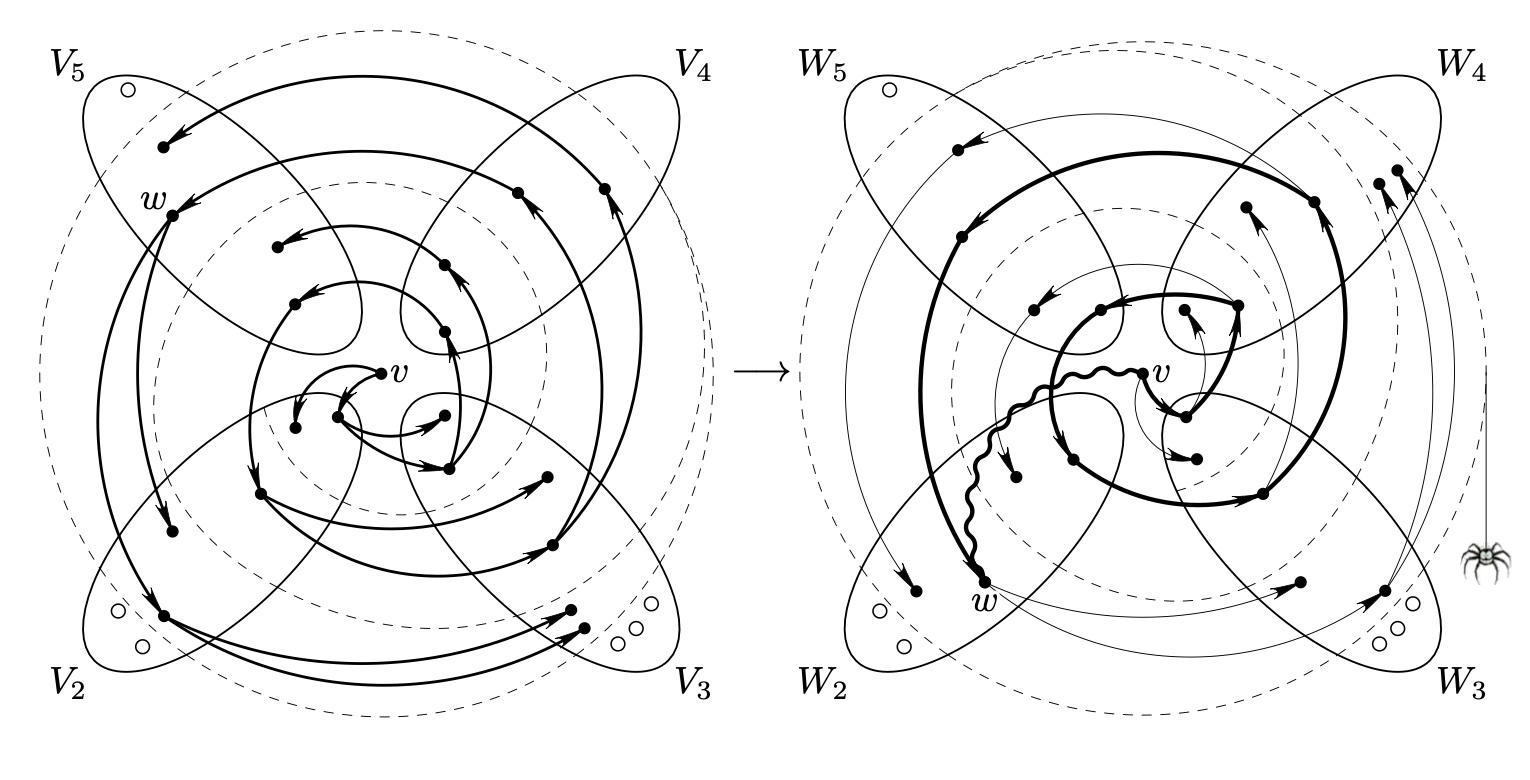
\includegraphics[width= 1\linewidth]{C7_SL2015IMO}
		\caption{\small\textit{\color{hoccungpi}Hình $3.$ Quy trình xây dựng chu trình.}}
		\vspace*{-10pt}
	\end{figure}
	Chú ý rằng, với cách đánh dấu các đỉnh, sau khi quy kết thúc; các đỉnh đã đánh dấu ở $V_i$ sẽ không có đỉnh kề trong $V_{i+1}$ mà đỉnh kề này lại chưa được đánh dấu. Hơn nữa, $v$ sẽ liên thông với tất cả các đỉnh được đánh dấu bởi một đường đi có hướng (đi theo chiều các mũi tên). 
	\vskip 0.1cm
	Bây giờ, ta chuyển mỗi đỉnh được đánh dấu thuộc tập $V_i$ sang tập $V_{i+1}$ (các đỉnh từ $V_i$ sang $V_{i+1}$ bây giờ sẽ được tô lại màu $i+1$ thay vì $i$). Theo nhận xét ở trên, ta thu được một cách tô màu mới vẫn thỏa mãn $2$ đỉnh kề nhau không cùng màu. Ký hiệu cách tô này là 
	\begin{align*}
		V_1 \cup W_2 \cup \dots \cup W_k.
	\end{align*}
	Quan sát rằng $v$ kề với một đỉnh $w \in W_2$ nào đó vì nếu không 
	\begin{align*}
		(V_1 \setminus \{v\}) \cup (W_2 \cup \{v\} ) \cup W_3 \cup \dots \cup W_k
	\end{align*}	
	sẽ là một cách tô màu mới mà rõ ràng  $|V_1 \setminus \{v\}| < |V_1|$, mâu thuẫn với cách chọn để ($1$) là một cách tô màu theo thứ tự. Nếu $w$ không được đánh dấu thì nghĩa là ban đầu $w \in V_2$. Nhưng khi đó ở bước đầu tiên của quy trình, đỉnh $w$ phải được đánh dấu và như vậy nó sẽ phải được chuyển sang $V_3$, nhưng điều này không xảy ra. Vì vậy $w$ là một đỉnh được đánh dấu và như vậy nó được chuyển từ $V_k$ sang $V_2$, nghĩa là ban đầu $w \in V_k$. 
	\vskip 0.1cm
	Cũng do $w$ được đánh dấu, tồn tại một đường đi có hướng từ $v$ đến $w$, ta thấy đường đi này đi xoay vòng qua tất cả các đỉnh thuộc $V_2,\dots,V_k$, vì thế có số cạnh chia hết cho $k-1$, vì nói riêng là một số chẵn. Chỉ cần nối thêm cạnh từ $w$ đến $v$; ta có ngay một chu trình có một số lẻ cạnh. Vậy ta đã xây dựng được một chu trình lẻ cạnh và có đủ $k$ màu và Bổ đề $2$ được chứng minh.
	\vskip 0.1cm
	Quay trở lại việc chứng minh Bổ đề $1$. Ta chọn một cách tô có thứ tự của $G$ như ($1$). Tương tự như trong Bổ đề $2$, ta đánh số các màu từ $1$ đến $k$. Với mọi tập con $C \subset \{1;2;\dots;k\}$ sao cho $|C|$ là số lẻ lớn hơn $1$, ta sẽ chỉ ra một chu trình đi qua một số lẻ đỉnh và có đủ tất cả các màu trong $C$. Tính chất này sẽ đảm bảo rằng: hai tập $C$ khác nhau cho hai chu trình khác nhau. Điều đó kéo theo Bổ đề $1$ được chứng minh, vì có đúng $2^{k-1} -k$ tập $C$ có lực lượng là số lẻ lớn hơn $1$. 
	\vskip 0.1cm
	Ký hiệu $V_C = \bigcup\limits_{c \in C} V_c$ và $G_C$ là đồ thị con của $G$ \textit{cảm sinh} từ $V_C$, nghĩa là đồ thị có có tập đỉnh là $V_C$ và hai đỉnh bất kỳ của $V_C$ kề nhau trong $G_C$ khi và chỉ khi chúng kề nhau trong $G$. Rõ ràng, cách tô màu $G$ bằng $k$ màu cảm sinh một cách tô màu $G_C$ bằng $|C|$ màu. Hơn nữa, cách tô màu này cũng là một cách tô màu tối ưu và theo thứ tự của $G_C$, vì nếu có một cách tô màu $(W_c)_{c \in C}$ khác  dùng ít màu hơn, hoặc dùng đúng $|C|$ màu và là một cách tô màu theo thứ tự của $G_C$; thì kết hợp cách tô $(W_c)_{c \in C}$ và cách tô các $V_i$ mà $ i \notin C$, ta sẽ thu được một cách tô màu tốt hơn, hoặc là một cách tô có thứ tự khác với  cách tô ($1$), vô lý!
	\vskip 0.1cm
	Từ đó, áp dụng Bổ đề $2$ cho đồ thị $G_C$ và cách tô màu theo thứ tự tương ứng là $(V_c)_{c \in C}$, ta thu được một chu trình lẻ và có đủ các màu trong $C$. Vậy Bổ đề $1$ được chứng minh và do đó bài toán được giải quyết.  
	\vskip 0.1cm
	Nói chung, những lời giải sử dụng mô hình đồ thị, đặc biệt là với những bài toán mà mô hình đồ thị được ẩn đi luôn đem lại hứng thú và sự phấn khích lớn. Đào sâu thêm, ta thấy rằng, dù mô hình đồ thị có thể giúp ta diễn đạt và hình dung bài toán trực quan hơn, nhưng trong một số trường hợp, điều đó là chưa đủ. Đôi khi, sau khi có được một mô hình đồ thị, ta còn cần phải phát hiện thêm các tính chất đặc biệt của đồ thị này. Tiếp theo, chúng ta cùng tìm hiểu hai loại đồ thị với cấu trúc đặc biệt. 
	\vskip 0.1cm
	$\pmb{3.}$ \textbf{\color{hoccungpi}Đồ thị lưỡng phân}	
	\vskip 0.1cm
	Khi gặp một đồ thị có rất nhiều cạnh và đỉnh, để nhìn thấy cấu trúc của đồ thị, thường ta sẽ phân hoạch tập đỉnh thành các tập con, sao cho mỗi cạnh của đồ thị có hai đầu thuộc hai tập con khác nhau. Một đồ thị mà tập đỉnh có thể được phân hoạch thành hai tập con có tính chất  như vậy được gọi là một đồ thị lưỡng phân, hay còn gọi là đồ thị hai phần.
	\vskip 0.1cm
	\textbf{\color{hoccungpi}Định nghĩa} $\pmb{3.1}$ (Đồ thị lưỡng phân)\textbf{\color{hoccungpi}.}
		Đồ thị $\pazocal{G}=(V,E)$ gọi là \textit{lưỡng phân} (hay \textit{hai phần}) nếu tập đỉnh $V$ có thể phân hoạch thành hai tập hợp $V_1, V_2$, sao cho mỗi cạnh của đồ thị $\pazocal{G}$ đều có một đầu mút thuộc $V_1$ và đầu mút còn lại thuộc $V_2$. 
	\begin{figure}[H]
		\vspace*{-5pt}
		\centering
		\captionsetup{labelformat= empty, justification=centering}
		\definecolor{cqcqcq}{rgb}{0.7529411764705882,0.7529411764705882,0.7529411764705882}
		\begin{tikzpicture}[scale=0.3, hoccungpi]
			\draw [rotate around={90.:(5.,9.5)}] (5.,9.5) ellipse (4.5cm and 3.7416573867739413cm);
			\draw [rotate around={90.:(17.,9.5)}] (17.,9.5) ellipse (4.5cm and 3.7416573867739413cm);
			\draw [line width=1.pt] (5.,12.)-- (17.,11.);
			\draw [line width=1.pt] (5.,8.)-- (17.,11.);
			\draw [line width=1.pt] (5.,10.)-- (17.,9.);
			\draw [line width=1.pt] (5.,6.)-- (17.,7.);
			\draw (4.48,4.92) node[anchor=north west] {$\mathbf{V_1}$};
			\draw (16.54,4.94) node[anchor=north west] {$\mathbf{V_2}$};
			\begin{scriptsize}
				\draw [fill=black] (5.,12.) circle (4.5pt);
				\draw [fill=black] (5.,10.) circle (4.5pt);
				\draw [fill=black] (5.,8.) circle (4.5pt);
				\draw [fill=black] (5.,6.) circle (4.5pt);
				\draw [fill=black] (17.,11.) circle (4.5pt);
				\draw [fill=black] (17.,9.) circle (4.5pt);
				\draw [fill=black] (17.,7.) circle (4.5pt);
			\end{scriptsize}
		\end{tikzpicture}
		\caption{\small\textit{\color{hoccungpi} Hình $4.$ Minh họa đồ thị lưỡng phân.}}
		\vspace*{-10pt}
	\end{figure}
	Đồ thị lưỡng phân có những tính chất tương đối dễ thấy. Ví dụ, nếu tập đỉnh  $V$ được phân hoạch thành hai tập hợp $V_1, V_2$, thì $
	\sum\limits_{v \in V_1} \text{deg} (v) =  \sum\limits_{v \in V_2} \text{deg} (v) = |E|.$ Ngoài ra, số cạnh của đồ thị lưỡng phân $\pazocal{G}$ không vượt quá $|V_1| |V_2|$. Khi dấu bằng xảy ra, ta còn gọi đồ thị $\pazocal{G}$ là một đồ thị lưỡng phân đầy đủ và ký hiệu là $K_{a,b}$, với $a,b$ lần lượt là số phần tử của $V_1$, $V_2$.
	Tiếp theo, ta có một định lý để kiểm tra một đồ thị có là đồ thị lưỡng phân hay không. 
	\vskip 0.1cm
	\textbf{\color{hoccungpi}Định lý} $\pmb{3.1}$ (Dấu hiệu nhận biết)\textbf{\color{hoccungpi}.} 
		Cho  $\pazocal{G} = (V,E)$ là một đồ thị liên thông. Khi đó, các phát biểu sau là tương đương:
		\vskip 0.1cm
		$1.$ Đồ thị $\pazocal{G}$ lưỡng phân.
		\vskip 0.1cm
		$2.$ Các đỉnh của đồ thị $\pazocal{G}$ có thể tô bằng hai màu, sao cho hai đỉnh kề nhau không cùng màu.
		\vskip 0.1cm
		$3.$ Đồ thị $\pazocal{G}$ không chứa chu trình có số cạnh là lẻ.
		\vskip 0.1cm
	\textit{Chứng minh.} Ta dễ thấy rằng phát biểu $(1)$ tương đương với phát biểu $(2)$ vì $\pazocal{G}$ lưỡng phân tương đương với việc tập đỉnh của nó được phân hoạch thành hai tập $A,B$ mà mọi cạnh của $\pazocal{G}$ đều có một đầu mút thuộc $A$, một đầu thuộc $B$; và ta có thể tô các đỉnh thuộc $A$ bằng màu đen và các đỉnh thuộc $B$ màu trắng.
	\vskip 0.1cm
	Tiếp theo, ta chứng minh từ $(2)$ suy ra $(3)$. Nếu các đỉnh của $\pazocal{G}$ có thể được tô bằng hai màu sao cho hai đỉnh kề nhau bất kỳ khác màu mà có một chu trình lẻ cạnh thì dọc theo chu trình này, các đỉnh có màu đan xen nhau, vì thế đỉnh đầu và đỉnh cuối cùng màu, vô lý!
	\vskip 0.1cm
	Đảo lại, nếu $\pazocal{G}$ không chứa chu trình có số lẻ cạnh, ta có thể tô màu các đỉnh của nó như sau. Chọn một đỉnh gốc $u$ và tô đen, với mỗi đỉnh $v$, lấy tùy ý một đường đi từ $u$ đến $v$ (đường đi này luôn tồn tại vì $\pazocal{G}$ liên thông). Nếu đường đi này độ dài chẵn thì tô $v$ màu đen, nếu lẻ thì tô $v$ màu trắng. Cách tô này không phụ thuộc vào việc lựa chọn đường đi nào, vì mọi đường đi từ $u$ đến $v$ phải cùng tính chẵn lẻ, nếu không  bằng cách ghép một đường đi độ dài chẵn với một đường đi độ dài lẻ, ta thu được một chu trình độ dài lẻ. Hơn nữa, có thể thấy ngay cách tô này đảm bảo hai đỉnh kề nhau không cùng màu. 
	\vskip 0.1cm
	\textit{Lưu ý.} Giả thiết đồ thị $\pazocal{G}$ liên thông chỉ giúp ta dễ dàng hơn trong việc trình bày chứng minh trên. Kết quả của định lý trên vẫn đúng nếu ta bỏ đi giả thiết $\pazocal{G}$ liên thông. Tiếp theo, ta cùng xét một số ví dụ minh họa. 
	\vskip 0.1cm
	\textbf{\color{hoccungpi}Ví dụ} $\pmb{3.1}$ (Olympic Canada năm $2019$)\textbf{\color{hoccungpi}.} 
	Cho $n \geq 3$ điểm trên mặt phẳng sao cho không có ba điểm nào thẳng hàng. Hai người chơi một trò chơi như sau. Họ luân phiên chơi. Ở mỗi lượt chơi, người đến lượt chọn hai điểm chưa được nối và nối chúng lại với nhau. Người đầu tiên tạo ra một chu trình có số cạnh là lẻ thua cuộc. Tìm tất cả các giá trị của $n$ sao cho người chơi đầu tiên có chiến lược thắng cuộc.  
	\vskip 0.1cm
	\textbf{\color{hoccungpi}Nhận xét. } Mô hình đồ thị là rất rõ trong bài toán này. Do bài toán đề cập đến chu trình lẻ cạnh, nên ta nghĩ đến cấu trúc đồ thị lưỡng phân.  
	\vskip 0.1cm
	\textit{Lời giải.} Gọi hai người chơi là $A, B$ và giả sử $A$ là người chơi đầu tiên.
	\vskip 0.1cm
	Ở mọi thời điểm, khi người chơi vẫn có thể nối thêm một đường, thì đồ thị $\pazocal{G}$ vẫn chưa chứa chu trình lẻ cạnh. Do đó, nó vẫn là đồ thị lưỡng phân. Vì vậy, nếu người chơi $P$ thua, nghĩa là ở lượt chơi tiếp theo, với mọi cách nối hai điểm chưa được nối với nhau, anh ta đều tạo ra một đồ thị không còn là đồ thị lưỡng phân. Nói cách khác, đồ thị $\pazocal{G}$ ở thời điểm đó phải là đồ thị lưỡng phân đầy đủ $K_{a,b}$; với $a,b$ là các số nguyên không âm thỏa mãn $a+b =n$. Vì vậy, số cạnh của $\pazocal{G}$ khi đó là $ab$.
	\vskip 0.1cm
	Để $A$ giành chiến thắng, rõ ràng $ab$ phải là số lẻ. Nếu $n$ lẻ, thì chắc chắn một trong hai số $a,b$ chẵn. Suy ra $ab$ chẵn, và $A$ sẽ thua. 
	\vskip 0.1cm
	Nếu $n$ chẵn, chúng ta dự đoán trạng thái cuối cùng của đồ thị $\pazocal{G}$ sẽ là $K_{n/2,n/2}$ nếu cả $A$ và $B$ đều chơi một cách tối ưu. Vì vậy, nếu $n \equiv 0$ (mod $4$) thì $a=b = n/2$ đều chẵn và $A$ thua. Nếu $n \equiv 2$ (mod $4$) thì $a=b=n/2$ đều lẻ và $A$ thắng. Bây giờ, chúng ta sẽ chứng minh dự đoán trên.
	\vskip 0.1cm
	Chúng ta sẽ gọi một đồ thị lưỡng phân liên thông là {\it cân bằng} nếu các tập đỉnh đen và trắng  của nó (như trong Định lý $3.1$) của nó có lực lượng bằng nhau. (Điều kiện liên thông đảm bảo rằng cách tô màu là duy nhất, sai khác hoán vị các màu.) Tổng quát, một đồ thị hai phần được gọi là cân bằng nếu mỗi thành phần liên thông có nhiều hơn $1$ đỉnh của nó là cân bằng.
	\vskip 0.1cm
	Chiến lược chơi của người thắng cuộc là đảm bảo rằng sau mỗi lần anh ta chơi, đồ thị luôn là cân bằng và nói riêng số các đỉnh độc lập luôn là số chẵn.
	\vskip 0.1cm
	\textit{Trường hợp $1$: $n \equiv 2 \pmod 4$.} Người chơi $A$ có thể sử dụng chiến lược sau đây để đưa $\pazocal{G}$ về dạng $K_{n/2,n/2}$, và giành chiến thắng. Nhắc lại rằng, khi trò chơi chưa kết thúc, đồ thị là lưỡng phân. Hiển nhiên rằng ở nước đi đầu tiên $A$ sẽ nối $2$ đỉnh nào đó lại với nhau và do đó sau nước đi này thì đồ thị là cân bằng và số đỉnh cô lập là số chẵn. Ở mỗi lượt chơi sau đó của mình, tùy theo cách chơi của $B$ mà $A$ sẽ có cách chơi tương ứng:
	\vskip 0.1cm
	$\bullet$ Nếu $B$ nối một đỉnh cô lập với một đỉnh $S$ nào đó thuộc một thành phần liên thông không tầm thường (của đồ thị cân bằng đang có sau nước đi của $A$) thì $A$ sẽ nối một đỉnh cô lập khác với một đỉnh $T$ thuộc thành phần liên thông đó sao cho $S$ và $T$ có màu khác nhau.
	\vskip 0.1cm
	$\bullet$ Nếu $B$ nối $2$ đỉnh cô lập với nhau, hoặc nối $2$ đỉnh khác màu của một thành phần liên thông, hoặc nối $1$ đỉnh của một thành phần liên thông với $1$ đỉnh của một thành phần liên thông khác thì sau nước đi của $B$, đồ thị vẫn là cân bằng (và có số đỉnh cô lập là số chẵn). Khi này, $A$ chỉ cần nối $2$ đỉnh cô lập (nếu có) hoặc $2$ đỉnh không cô lập bất kỳ miễn là chúng không cùng màu.
	\vskip 0.1cm
	Ta dễ dàng kiểm tra được rằng cách chơi của $A$ đảm bảo rằng đồ thị luôn là cân bằng và đồ thị cuối cùng mà anh ta nhận được là $K_{n/2, n/2}$. 
	\vskip 0.1cm
	\textit{Trường hợp $2$: $n\equiv 0\pmod 4$.} Người chơi $B$ có thể sử dụng chiến lược giống hệt người chơi $A$ để đưa $\pazocal{G}$ về dạng  $K_{n/2,n/2}$, và giành chiến thắng.      
	\vskip 0.1cm
	Vậy người chơi $A$ có chiến lược  thắng khi và chỉ khi $n$ chia $4$ dư $2$.  
	\vskip 0.1cm
	\textbf{\color{hoccungpi}Ví dụ $\pmb{3.2}$} (Olympic Trung Quốc năm $2021$)\textbf{\color{hoccungpi}.}
	Một hội nghị có $n>3$ nhà khoa học, một số họ là bạn của nhau (quan hệ bạn bè là hai chiều và không có ai là bạn của chính bản thân mình). Người ta nhận thấy rằng, với mọi cách phân hoạch các nhà khoa học thành hai tập hợp khác rỗng, luôn tồn tại  hai người cùng thuộc một tập là bạn của nhau và hai người không cùng thuộc một tập là bạn của nhau.
	\vskip 0.1cm
	Trong ngày đầu tiên, mỗi nhà khoa học đưa ra một số nguyên không âm. Ở ngày thứ $k$, mỗi nhà khoa học thay đổi con số của mình bằng phần nguyên của trung bình cộng của các số của tất cả các bạn của mình trong ngày $k-1$. Chứng minh rằng, sau một số hữu hạn ngày, tất cả các nhà khoa học sẽ cùng đưa ra một con số.    
	\vskip 0.1cm
	\textit{Lời giải.}
	Chúng ta sẽ sử dụng mô hình đồ thị $\pazocal{G} = (V,E)$, trong đó mỗi nhà khoa học là một đỉnh và hai đỉnh nối với nhau nếu hai nhà khoa học này là bạn của nhau. Ta có $7$ nhận xét nhỏ như sau:
	\vskip 0.1cm
	$1.$ Đồ thị $\pazocal{G}$ liên thông. Thật vậy, giả sử $\pazocal{G}$ có ít nhất hai thành phần liên thông; gọi $S$ là một trong các thành phần liên thông. Xét phân hoạch $(V, V \setminus S)$: phân hoạch này không chứa hai người khác tập nhưng là bạn của nhau, mâu thuẫn.
	\vskip 0.1cm
	$2.$ Đồ thị $\pazocal{G}$ không là đồ thị lưỡng phân, vì nếu nó là đồ thị lưỡng phân thì ta phân hoạch tập đỉnh thành hai phía tương ứng. Khi đó, sẽ không tồn tại hai người là bạn của nhau cùng thuộc một tập. Điều này kéo theo đồ thị $\pazocal{G}$ phải chứa chu trình có số lẻ cạnh. Gọi một chu trình như vậy là $(P)$. 
	\vskip 0.1cm
	$3.$  Nhận xét trên kéo theo, giữa hai đỉnh bất kỳ $u,v$, tồn tại một đường đi từ $u$ đến $v$ có một số chẵn cạnh. Thật vậy, lấy một đỉnh $w$ thuộc chu trình $(P)$. Xét một đường đi có dạng $u-w-v$. Nếu đường đi này có một số chẵn cạnh thì ta có điều phải chứng minh; nếu nó có một số lẻ cạnh thì ta xét đường đi $u-w(P)w-v$, nghĩa là đường đi như trên, bổ sung thêm đường đi quanh $w$ bằng chu trình $(P)$: vì $(P)$ có một số lẻ cạnh nên nên đường đi này có một số chẵn cạnh. 
	\vskip 0.1cm
	$4.$ Xét dãy $(a_n)$, trong đó $a_n$ là số lớn nhất ở ngày thứ $n$. Dãy này  không tăng. Thật vậy, giả sử các nhà khoa học ở ngày thứ $n$ có số lớn nhất là $a_n$. Khi đó ở ngày $n+1$, mỗi nhà khoa học có số mới là trung bình cộng của các bạn của mình nên nó nhỏ hơn hoặc bằng $a_n$.
	\vskip 0.1cm
	$5.$  Mặt khác, dãy số nguyên $(a_n)$ bị chặn dưới bởi $0$, nên nó có giới hạn bằng $M$. Điều này có nghĩa là kể từ ngày thứ $N$ đủ lớn nào đó, ta luôn có $a_n = M$ với mọi $n \geq N$. 
	\vskip 0.1cm
	$6.$  \textit{Kể từ ngày thứ $N$, tất cả các nhà khoa học đều có số là $M$.} Để chỉ ra điều đó, ta sử dụng phương pháp phản chứng. Giả sử tồn tại nhà khoa học $v$ có số nhỏ hơn $M$ ở ngày thứ $k>N$, khi đó ở ngày thứ $k+1$, số của tất cả các bạn của $v$ sẽ nhỏ hơn $M$. Gọi khoảng cách giữa $2$ đỉnh (của một đồ thị liên thông) là số cạnh của đường đi ngắn nhất (sử dụng ít cạnh nhất) giữa chúng, ta sẽ có một dãy các sự kiện ở các ngày tiếp theo như sau:
	\vskip 0.1cm
	$\bullet$ Ở ngày $k+1$, tất cả các đỉnh có khoảng cách bằng $1$ đến $v$ đều có  số nhỏ hơn $M$.
	\vskip 0.1cm
	$\bullet$ Ở ngày $k+2$, tất cả các đỉnh có khoảng cách bằng $0,2$ đến $v$ đều có  số nhỏ hơn $M$.
	\vskip 0.1cm
	$\bullet$ Ở ngày $k+3$, tất cả các đỉnh có khoảng cách bằng $1,3$ đến $v$ đều có số nhỏ hơn $M$.
	\vskip 0.1cm
	\dots
	\vskip 0.1cm Ở ngày $k+2l$, tất cả các đỉnh có khoảng cách bằng $0,2,\dots,2l$ đến $v$ đều có số nhỏ hơn $M$.
	\vskip 0.1cm  
	$7.$ Tuy nhiên, vì giữa hai đỉnh $u,v$ bất kỳ đều tồn tại một đường đi có số chẵn cạnh, nên với $l$ đủ lớn, ở ngày $k+2l$, tất cả các nhà khoa học đều có số nhỏ hơn $M$, mâu thuẫn!!!  
	\vskip 0.1cm 
	Như vậy, ta có điều cần chứng minh.
	\vskip 0.1cm
	Trong các đồ thị lưỡng phân, có một loại đồ thị đặc biệt. Ỏ phần tiếp theo, ta sẽ cùng tìm hiểu loại đồ thị này. 
	\vskip 0.1cm
%	$\pmb{4.}$ \textbf{\color{hoccungpi}Đồ thị cây}
%	\vskip 0.1cm
%	Trong một số tình huống, ta có thể gặp những đồ thị mà số cạnh rất ít (còn gọi là đồ thị thưa). Khi đó, cấu trúc \textit{đồ thị cây} thường sẽ xuất hiện. Ta có định nghĩa về đồ thị cây như sau.
%	\vskip 0.1cm
%	\textbf{\color{hoccungpi}Định nghĩa} $\pmb{4.1}$ (Cây)\textbf{\color{hoccungpi}.}
%	Một đồ thị được gọi là một \textit{cây} nếu nó liên thông và không chứa một chu trình nào. 
%	\begin{figure}[H]
%		\vspace*{-5pt}
%		\centering
%		\captionsetup{labelformat= empty, justification=centering}
%		\definecolor{qqqqff}{rgb}{0.,0.,1.}
%		\begin{tikzpicture}[scale=0.4, hoccungpi]
%			\clip(3.52,0.5) rectangle (17.14,10.78);
%			\draw [line width=1.2pt] (9.,1.)-- (9.,4.);
%			\draw [line width=1.2pt] (9.,4.)-- (6.,7.);
%			\draw [line width=1.2pt] (6.,7.)-- (4.,10.);
%			\draw [line width=1.2pt] (6.,7.)-- (8.,10.);
%			\draw [line width=1.2pt] (9.,4.)-- (12.,10.);
%			\draw [line width=1.2pt] (9.,4.)-- (15.,7.);
%			\draw [line width=1.2pt] (15.,7.)-- (13.,10.);
%			\draw [line width=1.2pt] (15.,7.)-- (16.,10.);
%			\begin{scriptsize}
%				\draw [fill=qqqqff] (9.,1.) circle (5pt);
%				\draw [fill=qqqqff] (9.,4.) circle (5pt);
%				\draw [fill=qqqqff] (6.,7.) circle (5pt);
%				\draw [fill=qqqqff] (4.,10.) circle (5pt);
%				\draw [fill=qqqqff] (8.,10.) circle (5pt);
%				\draw [fill=qqqqff] (12.,10.) circle (5pt);
%				\draw [fill=qqqqff] (9.,4.) circle (5pt);
%				\draw [fill=qqqqff] (15.,7.) circle (5pt);
%				\draw [fill=qqqqff] (13.,10.) circle (5pt);
%				\draw [fill=qqqqff] (16.,10.) circle (5pt);
%			\end{scriptsize}
%		\end{tikzpicture}
%		\caption{\small\textit{\color{hoccungpi} Hình $5.$ Minh họa đồ thị cây.}}
%		\vspace*{-10pt}
%	\end{figure}
%	Lưu ý rằng, một đồ thị cây không chứa chu trình, do đó nó không thể chứa một chu trình lẻ cạnh, hay một đồ thị cây cũng đồng thời là một đồ thị lưỡng phân. Nếu đồ thị $\pazocal{G}$ gồm một số thành phần liên thông, mà mỗi thành phần liên thông là một cây, thì $\pazocal{G}$ còn được gọi là một \textit{rừng}. Ta có định lý sau:
%	\vskip 0.1cm 
%	\textbf{\color{hoccungpi}Định lý} $\pmb{4.1}$ (Các đặc trưng tương đương của cây)\textbf{\color{hoccungpi}.}
%	Cho  $\pazocal{G}$ là một đồ thị có $n$ đỉnh. Khi đó, các phát biểu sau là tương đương:
%	\vskip 0.1cm
%	$1.$ $\pazocal{G}$ là một cây;
%	\vskip 0.1cm
%	$2.$ $\pazocal{G}$ không có chu trình và có $n-1$ cạnh;
%	\vskip 0.1cm
%	$3.$ $\pazocal{G}$ liên thông và có $n-1$ cạnh;
%	\vskip 0.1cm
%	$4.$ $\pazocal{G}$ không có chu trình và nếu bổ sung vào một cạnh nối hai đỉnh không kề nhau thì xuất hiện một chu trình duy nhất;
%	\vskip 0.1cm
%	$5.$ $\pazocal{G}$ liên thông và nếu bỏ đi một cạnh bất kỳ thì $\pazocal{G}$ mất tính liên thông;
%	\vskip 0.1cm
%	$6.$ Mỗi cặp đỉnh trong $\pazocal{G}$ được nối với nhau bằng một đường đi duy nhất.
%	\vskip 0.1cm
%	Việc chứng minh định lý trên không khó. Bạn đọc quan tâm có thể tìm hiểu chi tiết chứng minh trong [$4$]. Để minh họa, chúng ta hãy cùng xét hai ví dụ sau.
%	\vskip 0.1cm
%	\textbf{\color{hoccungpi}Ví dụ} $\pmb{4.1}$ (Bài toán dự tuyển thi IMO  năm $2019$, Croatia đề xuất)\textbf{\color{hoccungpi}.}
%	Trong một mạng xã hội, có $2019$ người dùng, một số họ là bạn của nhau (quan hệ bạn bè là quan hệ $2$ chiều). Ban đầu, có $1010$ người mà mỗi người có đúng $1009$ bạn và có $1009$ người mà mỗi người có đúng $1010$ bạn. Tuy nhiên, quan hệ bạn bè trong mạng này không bền vững, những sự kiện tương tự như sự kiện sau có thể lần lượt xảy ra (mỗi thời điểm chỉ có đúng một sự kiện xảy ra):
%	\vskip 0.1cm
%	Ký hiệu $A,B,C$ là ba người dùng sao cho $A$ là bạn của cả $B$ và $C$, nhưng $B$ và $C$ không phải là bạn của nhau. Khi đó $B$ và $C$ sẽ trở thành bạn, đồng thời $A$ không còn là bạn của cả $B$ và $C$.
%	\vskip 0.1cm
%	Chứng minh rằng, với mọi cấu hình ban đầu, tồn tại một dãy các sự kiện như sự kiện trên mà sau đó, mỗi người dùng chỉ còn tối đa một người bạn.  
%	\vskip 0.1cm
%	\textbf{\color{hoccungpi}Nhận xét. } Bài toán trên rõ ràng có thể phát biểu lại bằng ngôn ngữ của lý thuyết đồ thị như sau. Cho một đồ thị $\pazocal{G}$ có $2019$ đỉnh. Trong đó, $1010$ đỉnh có bậc $1009$ và $1009$ đỉnh có bậc $1010$. Ở mỗi bước, ta có thể: \textit{``Chọn ra ba đỉnh $A,B,C$ mà $A$ nối với cả $B$ và $C$; còn $B,C$ không nối với nhau. Sau đó, xóa hai cạnh $AB,AC$ và thêm cạnh $BC$ vào đồ thị $\pazocal{G}$.''}
%	\vskip 0.1cm
%	Gọi mỗi thao tác trên là một thao tác \textit{đảo cạnh}. Ta cần chứng minh rằng, thông qua một dãy các thao tác đảo cạnh, ta có thể tạo ra một đồ thị mà mỗi đỉnh của đồ thị có bậc không vượt quá $1$. Không khó để nhận ra, đây chính là một đồ thị rừng. 
%	\vskip 0.1cm
%	\textit{Lời giải.}
%	Chú ý rằng một thao tác đảo cạnh bảo toàn tính chất: đồ thị $\pazocal{G}$ có ít nhất một đỉnh bậc lẻ và không phải là một đồ thị đầy đủ (tính chất này là hiển nhiên). Ta cũng chú ý rằng, đồ thị ban đầu là liên thông (chứng minh được dành cho bạn đọc như một bài tập). Bây giờ, ta mô tả một thuật toán gồm hai bước để chuyển đồ thị ban đầu về một đồ thị mà bậc của mỗi đỉnh không vượt quá $1$. 
%	\vskip 0.1cm
%	\textit{Bước $1$: Tồn tại một dãy các thao tác đảo cạnh để chuyển đồ thị ban đầu về một đồ thị dạng cây.}
%	\vskip 0.1cm
%	\textit{Chứng minh.} Vì số cạnh của đồ thị giảm đi $1$ sau mỗi thao tác đảo cạnh, ta chỉ cần chứng minh: chừng nào đồ thị $\pazocal{G}$ còn chứa một chu trình, thì tồn tại một thao tác đảo cạnh sao cho đồ thị mới được tạo ra vẫn liên thông. Ta đi chứng minh đồ thị chứa một chu trình $\pazocal{Z}$ và các đỉnh $A,B,C$ sao cho hai đỉnh $A$ và $B$ kề nhau trong chu trình $\pazocal{Z}$, đỉnh $C$ không nằm trong chu trình $\pazocal{Z}$ và kề với đỉnh $A$ nhưng không kề với đỉnh $B$. Bỏ hai cạnh $AB, AC$ và thêm cạnh $BC$ sẽ bảo toàn tính liên thông của đồ thị và khẳng định được chứng minh.  
%	\begin{figure}[H]
%		\vspace*{-5pt}
%		\centering
%		\captionsetup{labelformat= empty, justification=centering}
%		\definecolor{qqqqff}{rgb}{0.,0.,1.}
%		\begin{tikzpicture}[scale=0.25,hoccungpi]
%			\draw (18.,30.)-- (12.,24.);
%			\draw (12.,24.)-- (18.,18.);
%			\draw (18.,18.)-- (26.,18.);
%			\draw (26.,18.)-- (32.,24.);
%			\draw (32.,24.)-- (26.,30.);
%			\draw (26.,30.)-- (18.,30.);
%			\draw (32.,24.)-- (38.,30.);
%			\draw [dash pattern=on 2pt off 2pt] (26.,30.)-- (38.,30.);
%			\draw (32.1,24.2) node[anchor=north west] {$A$};
%			\draw (25.5,32) node[anchor=north west] {$B$};
%			\draw (37.6,32) node[anchor=north west] {$C$};
%			\begin{scriptsize}
%				\draw [fill=qqqqff] (18.,30.) circle (5pt);
%				\draw [fill=qqqqff] (12.,24.) circle (5pt);
%				\draw [fill=qqqqff] (18.,18.) circle (5pt);
%				\draw [fill=qqqqff] (26.,18.) circle (5pt);
%				\draw [fill=qqqqff] (32.,24.) circle (5pt);
%				\draw [fill=qqqqff] (26.,30.) circle (5pt);
%				\draw [fill=qqqqff] (38.,30.) circle (5pt);
%			\end{scriptsize}
%		\end{tikzpicture}
%		\caption{\small\textit{\color{hoccungpi}Hình $6.$ Nếu đồ thị $\pazocal{G}$ chứa chu trình $\pazocal{Z}$, thì ta vẫn có thể giảm số cạnh của nó.}}
%		\vspace*{-10pt}
%	\end{figure}
%	Để tìm chu trình $\pazocal{Z}$ và các đỉnh $A,B,C$; ta sử dụng hai chiến lược sau. Nếu đồ thị $\pazocal{G}$ chứa một tam giác, ta xét một đồ thị con đầy đủ lớn nhất $K$. Rõ ràng $K$ chứa ít nhất ba đỉnh. Vì đồ thị $\pazocal{G}$ không là đồ thị đầy đủ, tồn tại một đỉnh $C$ không thuộc $K$ và kề với một đỉnh $A$ thuộc $K$. Do tính lớn nhất của $K$, có một đỉnh $B$ thuộc $K$ không kề với đỉnh $C$, và do đó ta có thể chọn chu trình $\pazocal{Z}$ trong $K$ và đi qua cạnh $AB$. 
%	\vskip 0.1cm
%	Nếu đồ thị $\pazocal{G}$ không chứa tam giác, ta xét một chu trình ngắn nhất $\pazocal{Z}$ trong đồ thị $\pazocal{G}$. Chu trình này không thể là một chu trình Hamilton (tức là chu trình đi qua tất cả các đỉnh của đồ thị, mỗi đỉnh đúng một lần). Thật vậy, nếu không, do tính nhỏ nhất của $\pazocal{Z}$, đồ thị $\pazocal{G}$ sẽ không chứa thêm một cạnh nào nữa, dẫn đến mỗi đỉnh của đồ thị $\pazocal{G}$ đều có bậc bằng $2$, mâu thuẫn với việc đồ thị luôn có đỉnh bậc lẻ. Như vậy, $\pazocal{Z}$ không là một chu trình Hamilton và vì thế có thể tìm được một đỉnh $C$ không thuộc $\pazocal{Z}$ và kề với một đỉnh $A$ thuộc $\pazocal{Z}$. Do đồ thị $\pazocal{G}$ không chứa tam giác, đỉnh $C$ sẽ không kề với bất kỳ đỉnh $B$ nào kề với $A$ trong $\pazocal{Z}$ và ta chọn được chu trình $\pazocal{Z}$ và ba đỉnh $A,B,C$.    
%	\begin{figure}[H]
%		\vspace*{-5pt}
%		\centering
%		\captionsetup{labelformat= empty, justification=centering}
%		\definecolor{qqqqff}{rgb}{0.,0.,1.}
%		\definecolor{cqcqcq}{rgb}{0.7529411764705882,0.7529411764705882,0.7529411764705882}
%		\begin{tikzpicture}[scale=0.25, hoccungpi]
%			\draw (18.,30.)-- (12.,24.);
%			\draw (12.,24.)-- (18.,18.);
%			\draw (18.,18.)-- (26.,18.);
%			\draw (26.,18.)-- (32.,24.);
%			\draw (32.,24.)-- (26.,30.);
%			\draw (26.,30.)-- (18.,30.);
%			\draw (32.,24.)-- (38.,30.);
%			\draw [dash pattern=on 2pt off 2pt] (26.,30.)-- (38.,30.);
%			\draw (32.1,24.2) node[anchor=north west] {$A$};
%			\draw (25.5,32) node[anchor=north west] {$B$};
%			\draw (37.6,32) node[anchor=north west] {$C$};
%			\draw (18.,30.)-- (26.,18.);
%			\draw (26.,30.)-- (18.,18.);
%			\draw (12.,24.)-- (32.,24.);
%			\draw (18.,30.)-- (18.,18.);
%			\draw (26.,30.)-- (26.,18.);
%			\draw (12.,24.)-- (26.,30.);
%			\draw (26.,18.)-- (12.,24.);
%			\draw (18.,30.)-- (32.,24.);
%			\draw (32.,24.)-- (18.,18.);
%			\begin{scriptsize}
%				\draw [fill=qqqqff] (18.,30.) circle (5pt);
%				\draw [fill=qqqqff] (12.,24.) circle (5pt);
%				\draw [fill=qqqqff] (18.,18.) circle (5pt);
%				\draw [fill=qqqqff] (26.,18.) circle (5pt);
%				\draw [fill=qqqqff] (32.,24.) circle (5pt);
%				\draw [fill=qqqqff] (26.,30.) circle (5pt);
%				\draw [fill=qqqqff] (38.,30.) circle (5pt);
%			\end{scriptsize}
%		\end{tikzpicture}
%		\caption{\small\textit{\color{hoccungpi} Hình $7.$ Minh họa cách tìm chu trình $\pazocal{Z}$ và ba điểm $A,B,C$.}}
%		\vspace*{-10pt}
%	\end{figure} 
%	\textit{Bước $2$: Mọi đồ thị dạng cây đều có thể chuyển về một đồ thị có bậc mỗi đỉnh không vượt quá $1$ thông qua một dãy các thao tác đảo cạnh.}
%	\vskip 0.1cm
%	\textit{Chứng minh.} Để ý rằng thao tác đảo cạnh  bảo toàn tính chất không chứa chu trình. Do đó, kể từ một cây, sau các thao tác đảo cạnh, ta luôn có một đồ thị không chứa chu trình. Ngoài ra, mỗi thao tác đảo cạnh sẽ giảm số cạnh của đồ thị đi $1$ nên  đến một lúc nào đó ta không thể thực hiện thêm một thao tác đảo cạnh nào nữa. Khi này bậc của mỗi đỉnh của đồ thị này không vượt quá $1$. Thật vậy, nếu có một đỉnh $A$ với  kề với hai đỉnh $B,C$ nào đó (khi đó $B,C$ không kề nhau vì đồ thị đang xét không chứa chu trình) thì ta có thể thực hiện thêm một thao tác đảo cạnh.
%	\vskip 0.1cm
%	\textbf{\color{hoccungpi}Ví dụ} $\pmb{4.2}$ (Kỳ thi chọn đội tuyển Mỹ tham dự Egmo $2020$)\textbf{\color{hoccungpi}.} Cho $\pazocal{G}=(V,E)$ là một  đồ thị đơn có $n$ đỉnh. Một cạnh $e$ của của nó được gọi là một \textit{cạnh cổ chai} nếu có thể phân hoạch $V$ thành hai  tập $A,B$ thỏa mãn:
%	\vskip 0.1cm
%	$1.$ Có tối đa $100$ cạnh của $\pazocal{G}$ có một đầu mút thuộc $A$ và đầu mút còn lại thuộc $B$;
%	\vskip 0.1cm
%	$2.$ Cạnh $e$ là một trong số các cạnh như vậy.
%	\vskip 0.1cm 
%	Chứng minh rằng đồ thị $\pazocal{G}$ có tối đa $100(n-1)$ cạnh cổ chai.
%	\vskip 0.1cm
%	\textbf{\color{hoccungpi}Nhận xét. } Con số $100(n-1)$ ít nhiều gợi ý cho ta $100$ cấu trúc cây trong đồ thị $\pazocal{G}$. 
%	\vskip 0.1cm
%	\textit{Lời giải.} Gọi $F_1$ là một rừng lớn nhất trong $\pazocal{G}$ (nếu $\pazocal{G}$ liên thông thì $F_1$ chính là một cây). Xóa đi các cạnh của $F_1$ và gọi $F_2$ là rừng lớn nhất trong đồ thị mới nhận được (vẫn có $n$ đỉnh). Cứ tiếp tục như vậy, cho đến $F_{100}$ là rừng lớn nhất trong đồ thị nhận được khi xóa đi các cạnh của  $F_1\cup F_2\cup \cdots \cup F_{99}$. Giả sử ngược lại, $\pazocal{G}$ có nhiều hơn $100(n-1)$ cạnh cổ chai. Mỗi rừng $F_i$ (với $i=1,\dots,100$) (có $n$ đỉnh) có tối đa $n-1$ cạnh. Do vậy, tổng số các cạnh trong $F_1\cup F_2\cup \cdots \cup F_{100}$ không vượt quá $100(n-1)$. Vì vậy, vẫn tồn tại một cạnh cổ chai không nằm trong bất kỳ $F_{i}, i=1, 2, \ldots, 100$ nào.
%	Gọi $x-y$ là một cạnh như vậy ($x,y$ là hai đỉnh của đồ thị). Rõ ràng, trong mỗi $F_i$, có một đường đi từ $x$ đến $y$ vì nếu không, thêm cạnh $x-y$ vào $F_i$ ta vẫn có một rừng (mâu thuẫn với cách chọn $F_i$ lớn nhất). Vì vậy, trong $\pazocal{G}$ có ít nhất $101$ đường đi từ $x$ đến $y$, hơn nữa hai đường đi bất kỳ đều không có cạnh chung. Tuy nhiên, khi đó cạnh $x-y$ không thể là cạnh cổ chai. Thật vậy, gọi $A,B$ là phân hoạch của $V$ tương ứng với cạnh cổ chai $x-y$. Với mỗi $i$, đường đi  trong $F_i$ từ $x$ đến $y$ phải chứa một cạnh nối một đỉnh thuộc $A$ và một đỉnh thuộc $B$. Tóm tại, ta tìm được $101$ cạnh của $G$ mà một đầu mút thuộc $A$ và  đầu mút còn lại thuộc $B$ (mâu thuẫn với điều kiện $(1)$). 
%	\vskip 0.1cm
%	Hy vọng rằng qua một số lý thuyết và bài tập minh họa, bạn đọc đã ít nhiều thấy được tiềm năng, sự phong phú và mối liên hệ của lý thuyết đồ thị với nhiều mảng kiến thức khác. Rõ ràng, khi mô hình hóa được một bài toán dưới dạng ngôn ngữ đồ thị, ta có thể tìm ra định hướng tốt trong việc tìm kiếm lời giải. Cụ thể hơn, khi gặp một mô hình đồ thị có nhiều cạnh, ta có thể liên tưởng đến cấu trúc đồ thị lưỡng phân; ngược lại, một mô hình đồ thị ít cạnh làm chúng ta liên tưởng đến đồ thị dạng cây, rừng.  
%	Phần cuối của bài viết này là một số bài tập giúp rèn luyện thêm kỹ năng phát hiện và sử dụng các cấu trúc đồ thị lưỡng phân và cây.   
%	\vskip 0.1cm
%	$\pmb{5.}$ \textbf{\color{hoccungpi}Một số bài toán tự rèn luyện}
%	\vskip 0.1cm
%	\textbf{\color{hoccungpi}Bài $\pmb{1.}$} \textit{(Olympic Canada năm $2020$)} Cho đồ thị $\pazocal{G}$ có $19998$ đỉnh. Mỗi đồ thị con gồm $9999$ đỉnh của $\pazocal{G}$ đều chứa ít nhất $9999$ cạnh. Hỏi $\pazocal{G}$ có ít nhất bao nhiêu cạnh?
%	\vskip 0.1cm
%	\textbf{\color{hoccungpi}Bài $\pmb{2.}$}\textit{(Mở rộng Bài $2$)}  Cho đồ thị $\pazocal{G}$ có $2n$ đỉnh. Mỗi đồ thị con $n$ đỉnh của  $\pazocal{G}$ đều có ít nhất $n$ cạnh. Chứng minh rằng $\pazocal{G}$ có ít nhất $5n$ cạnh.
%	\vskip 0.1cm
%	\textbf{\color{hoccungpi}Bài $\pmb{3.}$} \textit{(Olympic Liên bang Nga năm $2004$)} Một quốc gia có $1001$ thành phố.  Hai thành phố bất kỳ được nối với nhau bằng một con đường một chiều. Mỗi thành phố có $500$ con đường đi ra và $500$ con đường đi vào. Có một tổ chức ly khai xuất hiện và chiếm đóng $668$ thành phố. Chứng minh rằng, trong khu vực ly khai này, từ mỗi thành phố đều có có thể đi đến một thành phố khác.
%	\vskip 0.1cm
%	\textbf{\color{hoccungpi}Bài $\pmb{4.}$}  Cho đồ thị $\pazocal{G} = (V,E)$ thỏa mãn $|E| = |V| +4$. Chứng minh rằng, trong $\pazocal{G}$ có
%	hai chu trình không có cạnh chung. 
	\vskip 0.1cm
	\textbf{\color{hoccungpi}Tài liệu}
	\vskip 0.1cm
	[$1$] Đỗ Đức Thái, \textit{Chuyên đề học tập toán $11$}. NXB Đại học Sư phạm Hà Nội. 
	\vskip 0.1cm
	[$2$] Hà Huy Khoái, \textit{Chuyên đề học tập toán $11$}. NXB Giáo dục Việt Nam. 
	\vskip 0.1cm
	[$3$] Asratian, Armen S.; Denley, Tristan M. J.; Häggkvist, Roland, \textit{Bipartite Graphs and their Applications}. Cambridge University Press, $1998$.
	\vskip 0.1cm
	[$4$] Bender, Edward A.; Williamson, S. Gill , \textit{Lists, Decisions and Graphs  With an Introduction to Probability}, $2010$.
	\vskip 0.1cm
	[$5$] Titu Andreescu, Bogdan Enescu, \textit{Mathematical Olympiad Treasures}. Springer, $2011$.
	\vskip 0.1cm                 
	[$6$] Website \url{https://artofproblemsolving.com}. 
\end{multicols}